\documentclass[a4paper, 12pt, twoside, openright]{mythesis}

\renewcommand{\baselinestretch}{1}       % for squeezing the draft into the page limit, do not use

% Note
% Use \textsc{Name} to separate images, videos, dataset names from the main texts.

% =============================================================================
% Commonly used packages
% =============================================================================

% For removing Package ifpdf Error
%%%%%%\let\ifpdf\relax

% For removing LaTeX Font Warning
\usepackage{lmodern}

% Add Reference in Contents
\usepackage[nottoc]{tocbibind}

% Figures
%\usepackage{subcaption}
\usepackage{float}
%\usepackage[justification=raggedright]{caption}	% makes captions ragged right - thanks to Bryce Lobdell
\usepackage{lscape} % Useful for wide tables or figures.
\usepackage{makecell}
\usepackage{sidecap}

\graphicspath{{figures}{example}}

% Algorithm
\usepackage[lined,ruled,linesnumbered]{algorithm2e}
\usepackage{algorithmic}

% Table and list
\usepackage{booktabs} % Publication quality tables
\usepackage{multirow}
\usepackage{rotating} % sideways
\newcommand{\vergap}[1]{\renewcommand{\arraystretch}{#1}}
\newcommand{\horgap}[1]{\setlength{\tabcolsep}{#1}}
%\specialrule{width}{abovespace}{belowspace}
\newcommand{\dtoprule}{\specialrule{2pt}{0pt}{2pt}}
\newcommand{\dbottomrule}{\specialrule{2pt}{0pt}{\belowrulesep}}
\usepackage{colortbl}

\usepackage{paralist}
\usepackage{enumitem}

% Math
\usepackage{bm} % Make bold, italic math symbols
\usepackage{epsfig} % for figures
\usepackage{graphicx} % another package that works for figures
\usepackage{times}
%\usepackage{mathptmx}
\usepackage{mathtools}
\usepackage{textcomp, gensymb} % math symbol
\usepackage{amssymb,amsmath,amsfonts} % Short math guide for LaTeX ftp://ftp.ams.org/pub/tex/doc/amsmath/short-math-guide.pdf
\usepackage{siunitx} % SI units
\newcommand{\norm}[1]{\left\lVert#1\right\rVert}
\newcommand{\cp}[1]{\left[#1\right]_{\times}}

% Fonts
\usepackage{units}
\usepackage{color}

% Comments
\usepackage{comment}

% Hyperlinks
\usepackage{url} % Hyphenation of URLs.
\usepackage{xcolor}
\usepackage[backref=page]{hyperref}
\hypersetup{colorlinks,breaklinks,
            urlcolor=[rgb]{0.918,0,0.545},
            linkcolor=[rgb]{0.710,0.180,0.141},
            citecolor=[rgb]{0,0.545,0.447}}
\usepackage{bookmark}
%\usepackage[pagebackref=true,breaklinks=true,colorlinks,bookmarks=false]{hyperref} % remove letterpaper=true,
%
\usepackage{slashbox}
\usepackage{xspace}
%\usepackage[table,caption=false]{xcolor}
%\usepackage{setspace}

% Better hyphenation
\usepackage{microtype}

% Appendix
\usepackage[toc,page]{appendix}

% =========================================
% Useful macros
% =========================================

% Latin abbreviations
\newcommand{\etal}{\textit{et al}.~} % ``and others'', ``and co-workers''
\newcommand{\eg}{e.g.,~} % ``for example''
\newcommand{\ie}{i.e.,~} % ``that is'', ``in other words''
\newcommand{\suchthat}{\, \mid \,}

% Math related
\DeclareMathOperator*{\argmin}{\arg\!\min}
\DeclareMathOperator*{\argmax}{\arg\!\max}
\DeclareMathOperator{\avg}{avg}
\DeclareMathOperator{\Tr}{Tr}

% Paragraph
\let\originalparagraph\paragraph
\renewcommand{\paragraph}[2][.]{\originalparagraph{#2#1}}

% Consistent margin adjustment for paragraphs, figures, and sections
\newlength\paramargin
\newlength\figmargin
\newlength\secmargin

\setlength{\secmargin}{0.0mm}
\setlength{\paramargin}{0.0mm}
\setlength{\figmargin}{0.0mm}

% References for figures, tables, equations, chapters, and sections
\newcommand{\chref}[1]{Chapter~\ref{ch:#1}}
\newcommand{\secref}[1]{Section~\ref{sec:#1}}
\newcommand{\figref}[1]{Figure~\ref{fig:#1}}
\newcommand{\tabref}[1]{Table~\ref{tab:#1}}
\newcommand{\eqnref}[1]{\eqref{eq:#1}}
\newcommand{\thmref}[1]{Theorem~\ref{#1}}
\newcommand{\prgref}[1]{Program~\ref{#1}}
\newcommand{\algref}[1]{Algorithm~\ref{#1}}
\newcommand{\clmref}[1]{Claim~\ref{#1}}
\newcommand{\lemref}[1]{Lemma~\ref{#1}}
\newcommand{\ptyref}[1]{Property~\ref{#1}}

% Comments
\long\def\ignorethis#1{}
\newcommand {\sychien}[1]{{\color{blue}\textbf{Po-Chen: }#1}\normalfont}
\newcommand {\coauthorA}[1]{{\color{red}\textbf{Co-author A: }#1}\normalfont}
\newcommand {\coauthorB}[1]{{\color{magenta}\textbf{Co-author B: }#1}\normalfont}
\newcommand {\todo}{{\textbf{\color{red}[TO-DO]\_}}}
\def\newtext#1{\textcolor{blue}{#1}}
\def\modtext#1{\textcolor{red}{#1}}

%\usepackage{ifthen}
%\ifthenelse{\equal{\final}{1}}
%{
%  \renewcommand{\sychien}[1]{}
%}
%{}

\newcommand{\tb}[1]{\textbf{#1}}
\newcommand{\mb}[1]{\mathbf{#1}}
\newcommand{\Paragraph}[1]{\noindent\textbf{#1}}

\newcommand{\jbox}[2]{
  \fbox{%
  	\begin{minipage}{#1}%
  		\hfill\vspace{#2}%
  	\end{minipage}%
  }
}

\newcommand{\jblock}[2]{%
  \begin{minipage}[t]{#1}\vspace{0cm}\centering%
  #2%
  \end{minipage}%
}
	
% Customized definition
\newcommand{\Ic}{\mathcal{I}_{c}}
\newcommand{\It}{\mathcal{I}_{t}}
\newcommand{\Ot}{\mathcal{O}_{t}}
\newcommand{\asin}{\mathrm{asin}}
\newcommand{\acos}{\mathrm{acos}}
\newcommand{\atan}{\mathrm{atan}}
\newcommand{\atanT}{\mathrm{atan2}}
\newcommand{\dotP}{\mathrm{dot}}


\renewcommand{\baselinestretch}{1.5}

%\hypersetup{
%    colorlinks=true,       % false: boxed links; true: colored links
%    linkcolor=blue,          % color of internal links
%    citecolor=blue,        % color of links to bibliography
%    filecolor=blue,      % color of file links
%    urlcolor=blue           % color of external links
%}

%------------------------------------
% Thesis boundary Setting
%-------------------------------------

\textwidth      = 137.0mm
\textheight     = 224.0mm
\topmargin      =  -3.0mm
\headheight     =   7.0mm
\headsep        =  10.0mm
\footskip       =   8.0mm
\oddsidemargin  =  10.6mm
\evensidemargin =  10.6mm
\hoffset = -0.2cm
%\overfullrule=5pt%%

\pagenumbering{roman}% \thispagestyle{myheadings}
\setcounter{page}{1}
%\thispagestyle{empty}

\begin{document}
\title{\textbf{Study for Robot-Assisted Endodontic Treatment}}

\author{ \\  \\ \\
{\it Yi-Chan Li}\\
{\it Advisor: Cheng-Wei Chen} \\ \\ \\ \\  \\ \\
{\it Graduate Institute of Electronics Engineering}\\
{\it National Taiwan University} \\
{\it Taipei, Taiwan}\\ }

{\date{May 2021}}

\maketitle

\frontmatter
\chapter{Abstract}
\label{ch:abstract}
\vspace*{-10mm}
\hspace*{6mm}Advancements in robot-assisted surgery invigorates researches on robotics in the dental field. Reviewing the literature on dental robots, this thesis aims to develop a root-assisted system for endodontic treatment to improve the success rate of surgery. Considering the workspace and extreme precision in endodontic treatment, our robot-assisted system - DentiBot consists of a robot arm, an F/T sensor. System integration solutions are examined in the thesis. Moreover, to overcome the two main failures of surgery - incomplete root preparation and instrument fracture, novel ideas to perform endodontic treatment with DentiBot are presented in this thesis. First, Force-guided alignment based on admittance control is involved to calibrate the surgical path in real-time. Second, file feedrate control is addressed to protect endodontic files from fracturing. Last but not least, an algorithm based on the above functions is proposed to achieve high performance in root preparation. The technical experiments have validated the feasibility of Force-guided alignment and a pre-clinical experiment has proved file feedrate control and our proposed algorithm.




\textit{Keywords: Endodontic treatment, Robot-assisted system, Admittance control, Force-guided alignment, File feedrate control, Instrument fracture}

 




\tableofcontents
\listoffigures
\listoftables

%------------------------------------
% Thesis Body -- begin
%------------------------------------

\mainmatter

\chapter{Introduction}
Endodontic treatment, also known as root canal treatment and nerve extraction, is performed to cure an infected tooth. The procedure of endodontic treatment is divided into three parts - Opening, Cleaning, and Filling shown in  Figure \ref{fig:endo-procedure}.
\begin{figure}[htbp]
\begin{center}
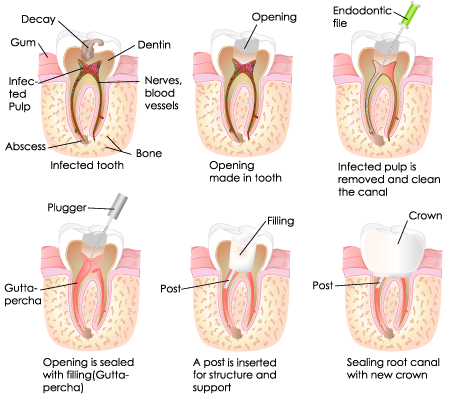
\includegraphics[width=0.8\linewidth]{Images/endo-procedure.png}
\end{center}
\caption{
The endodontic therapy steps
}\label{fig:endo-procedure}
\end{figure}
\newpage
An infected tooth results from periodontal disease, attrition, trauma, or decay. Once the dental pulp is infected, it causes an irreversible inflammation and let patients confront a root canal treatment. Figure \ref{fig:endo-procedure} shows an infected tooth and its dental pulp, which is composed of blood vessels, nerves, connective tissues, and lymphatics. In the "Opening" step, an experienced dentist drills the crown of infected tooth to remove the dentin and expose the infected pulp inside the canal to the air. Next, in the "Cleaning" step the dentist uses an endodontic file which is a flexible reamer to remove the infected pulp. Then, in the "Filling" step the dentist uses a dental plugger to fill the empty root canal with Gutta-percha which is a plastic substance. "Filling" can prevent cross infection between root canals because the cured teeth remains many invisible and inaccessible pulp tissue. Finally the dentist seals root canal with new crown to protect cured root canal. 
\par
"Cleaning" is of paramount importance in a whole treatment because untreated cleaning will result in pulp necrosis, apical abscess, periodontal ligament inflammation, or even cellulitis. If there are many remained infected pulp after root canal treatment, the surgery should be operated on again.
\section{Motivation}
The performance of the endodontic treatment depends on the dentist's own long-term experience. A qualified dentist can operate the endodontic treatment and accumulate their experience to increase the success rate. With many experiences, dentists can acquire an endodontist license. According to statistics from the Ministry of Health and Welfare, R.O.C. (Taiwan), the number of dentists in Taiwan is $15,178$. However, according to The Academy of Endodontology, R.O.C. (Taiwan), there are only $238$ dentists to acquire an endodontist license due to the expertise of endodontics. Besides, Root canal treatment is tedious and time-consuming due to complicated conditions of each tooth, a patient who suffered from an infected tooth spends much time see a dentist It takes at least two to three rounds, even spends more than two months in the worst case. 
\par
Therefore, our team looks forward to designing a robot-assisted system to help a dentist finish the root canal treatment. With the system, we wish it can increase the success rate for dentists and provide patients a safe surgery.

\section{Previous Work and Problem Definition}
(Previous work: briefly mention the existing dental robots)
\par\noindent
(Problem definition:
1.	Assist dentists to operate RCT and focus on cleaning procedure
2.	Root canal cannot be visually observed and is too small to clean well
3.	Risk of file breakage)		
\par\noindent
Instruments fracture and perforation are two problems that commonly occur during the therapy. Removal of broken files is both technically difficult and therefore it is important to reduce the probability of fracture. In addition, root canal treatment also requires repeatedly drilling in order to clean the canal thoroughly.  This repetitive action of root canal treatment is tedious and time-consuming. Therefore, we designed an automatic endodontic robot to improve the time-efficiency and to reduce the occurrence of instrument fracture in endodontic surgery.
The root canal cleaning is a big challenge in and of itself
There is one robotic system that is designed to perform endodontic therapy. In Intelligent Micro Robot Development for Minimum Invasive Endodontic Treatment [3] , they proposed a micro robot performing root canal treatment with the assistance of 3D computer model system. It is designed to accomplish endodontic therapy with path planned according to the 3D model. However, the problem of instruments fracture still remains. 
In this paper, a torque monitoring method is proposed. The main causes of fractured files are torsional fracture and flexural fatigue, account for 55.7\% and 44.3\% separately [5]. Therefore, we use current feedback to keep track of the torque which the file is bearing during the endodontic treatment. This torque monitoring system is implemented on an endodontic robot prototype we built. We primarily focus on the cleaning and shaping step since it’s the key step to a successful root canal treatment. With the robot prototype and torque monitoring system, the possibility of instrument fracture can be reduced. Besides, the repetitive action during the drilling step can be performed by the robot.			
\section{The Proposed Method}
(Solutions: (be consistent with problem definition)
1.	Build a robot-assisted system and enable it to drill
2.	Force-guided alignment 
3.	Control the file rotation speed
B.	Prospect:
\par\noindent
(Prospect: Move to the infected teeth$\longrightarrow $Root canal searching$\longrightarrow $Repetitive drilling$\longrightarrow $Apex Detection)						
\section{Main Contributions of the Thesis}
\begin{enumerate}
	\item	Integrate a 6-DoF robotic manipulator with 6-DoF F/T sensor for performing endodontic treatment.
	\item	Develop a framework for robot alignment regarding the position and orientation of root canal. 
	\item	Protect the endodontic file from fracturing by controlling file rotation speed.
\end{enumerate}
\section{Organization of the Thesis}
\chapter{Related Work and Literature Review}
(Elaborate more details of NCTU paper, YOMI and even other dental robots)			\\
(Why not Image processing and why force feedback?)								
\chapter{Robot-Assisted System}
\section{Requirement and Specification}
(Payload, resolution and workspace)														\\
(Why not RCM mechanism)																	
\section{System Design- The DentiBot}
(Why Robot Arm - Meca500, F/T sensor - Mini40, Customized Handpiece)					\\
(DOF discussion)																		
\chapter{Kinematics Analysis and Admittance Control}
(Tutorial, only variables without numbers and data) 													\\
(cite some technical papers)						
\section{Kinematics Analysis}
\subsection{Coordinate Definition}
(0~6 robot frame, Sensor frame, and tool frame)
\subsection{Forward and Inverse Kinematics}
--
\subsection{Jacobian matrix} 
(variables are shown in appendix because they are too long)												\\
(How to obtain Jacobian matrix in frame 6 by Jacobian matrix in frame 0)								
\subsection{Tool Center Point}
(How to find RCM by four-points-method)
\section{Admittance Control}
\subsection{Gravity Compensation}
\subsection{Admittance Control based on F/T sensor}
\subsubsection{Control Scheme}
(Block diagram, robot command choice)
\subsubsection{Discussion about Affection of Parameter Setting}
(K, Bi, Mi)
\subsection{Reference Frame Changing of F/T sensor}
(How to find the direction vector of the tool)															\\
(From sensor frame to tool tip frame)
\chapter{Self-Alignment of Root Canal Direction for Automatic Navigation}
\section{Problem Definition}
(Main cause of surgical failure)
\section{The Proposed Method}
(Peg-in-hole method based on F/T feedback)
\section{The Implementation of the method}
(What functions should we used to implement this method)\\
(Admittance control + Transformation from robot to tool \\
+ Transformation from sensor to tool					\\
+ Motion Planning: based on admittance control)														
\newpage
\section{Parameters Setting}
(get reasonable and suitable parameters first)			\\
(Modes: Doctor Dragging and Auto navigation)																							
\chapter{Precaution of Endodontic Files Fracture Based on Current Feedback}
\section{Problem Definition}
(Main cause of Files Fracture)					\\
(File property)
\section{The Proposed Method and Theorem}
(CACS2020)(Prototype 1)							\\
(Motion Planning: sections)(Current threshold setting)
\chapter{Preliminary Experiment Result}
\section{Experimental Setup}
(Communication protocol – EtherCAT, RTOS – NI target)						\\
For 7.2 experiment: (Stewart-Platform + PhaseSpace + markers)				\\
For 7.3 7.4 experiments: (Acrylic root canal model + truth tooth)
\section{Admittance Control}
(Metrics: position comparison between the target and the robot)
\section{Automatically Direction Changing}
(Metrics: time, completeness and file breakage)								\\
(Completeness definition: comparison of pixel area before and after experiment via image)
\section{Repetitive Experiment}
(Metrics: file breakage, compare with and without reverse)
\chapter{Conclusions and Future works}
(Patient move tracking via cable, root canals searching)
%------------------------------------
% Thesis Body -- end
%------------------------------------

\bibliographystyle{IEEEtran}
\bibliography{thesis}
\end{document}
